% !TeX root = ../report.tex
\section{Introduction}

\subsection{regular introduction stuff}

\subsection{Introduction to reinforcement learning}
Reinforcement learning is a machine learning paradigm dedicated to solving sequential decision processes. The definition of a reinforcement learning algorithm given by \citet{RLBook2018}, is an algorithm which can solve a specific kind of sequential decision problem, namely those which can be described formally by a \textit{finite Markov decision process}.


\subsubsection{Finite Markov Decision Processes}

The Markov decision process provides a formal description of sequential decision problems. 
In this project, we define a Markov decision process by a 4-tuple $(\mathcal{S},\mathcal{A},\mathcal{R}, p)$, where $\mathcal{S}$ is the state-space, $\mathcal{A}$ is the action-space, $\mathcal{R} \subset \mathbb{R}$ is the reward-space, and the function $p : \mathcal{S} \times \mathcal{R} \times \mathcal{S} \times \mathcal{A} \rightarrow \mathbb{R}$ describes the conditional probability of entering a state $s' \in \mathcal{S}$ with reward $r \in \mathcal{R}$ given the previous state was $s \in \mathcal{S}$ and action $a \in \mathcal{A}$ was chosen.
In finite Markov decision processes $\mathcal{S}$, $\mathcal{A}$ and $\mathcal{R}$ are all finite sets. 

\begin{align}
    \sum_{s' \in \mycal{S}}\sum_{r \in \mycal{R}} p(s', r, s, a) = 1 \qquad \forall s \in \mycal{S}, \forall a \in \mycal{A}(s)
\end{align}

\vspace*{0.5cm}

When solving Markov decision processes, a sequence of random variables is introduced. Let $T = \set{1, 2, \ldots}$ be a sequence of discrete time steps, $S_t$ is then a random variable which indicates the state of the environment at time step $t$, $A_t$ is the action chosen at time step $t$, from the set $\mathcal{A}(s)$ which denotes the actions available from state $s$. 
$R_t$ is the reward received after choosing action $A_{t-1}$ in state $S_{t-1}$

\vspace*{0.5cm}

\Cref{fig:agent-environment} visualises the agent-environment loop. 
Initially, the agent in placed in some environment \mycal{E}, from where the agent observes $S_0$.
The agent the chooses some an action, yielding $A_0$, after the action has been performed, state $S_{t+1}$ and $R_t$ is presented to the agent, this results in a sequence of the form $S_0,A_0,R_1,S_1,A_1,R_2,S_2,\ldots$



\begin{align*}
    p(s',r | s,a) \defeq \Pr{S_t\!=\!s', R_t\!=\!r | S_{t-1}\!=\!s, A_{t-1}\!=\!a}
\end{align*}

\begin{figure}[!htb]
    \centering
    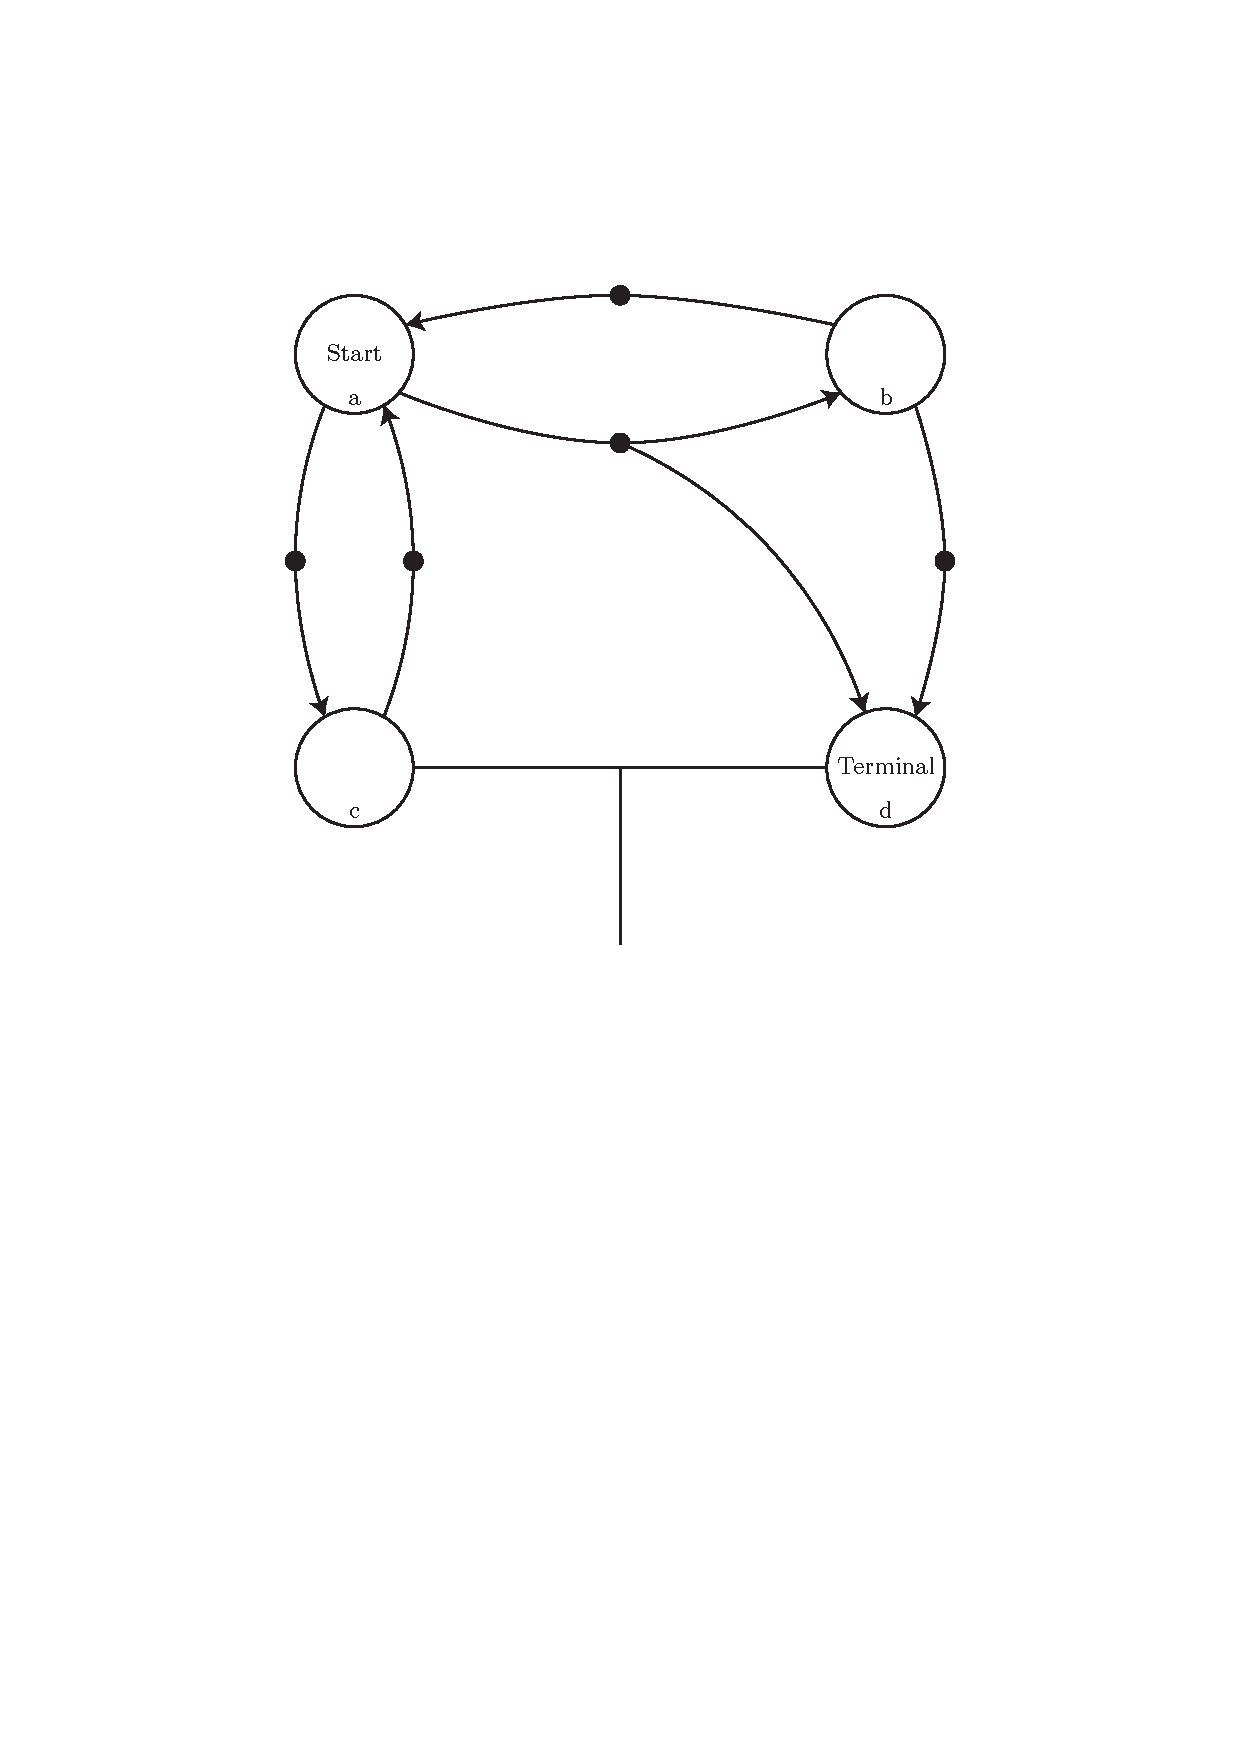
\includegraphics[scale=0.5]{../include/MDP.pdf}
    \caption{\todo}
    \label{fig:MDP}
\end{figure}

\begin{figure}[!htb]
    \centering
    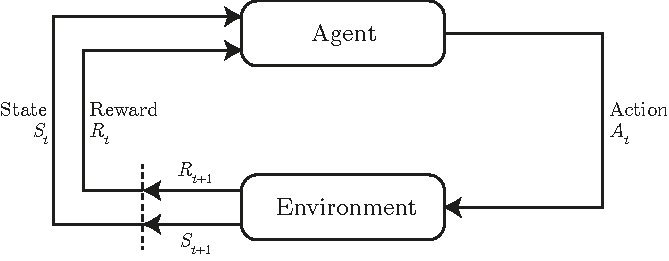
\includegraphics[scale=1]{../include/agent-environment-loop.pdf}
    \caption{The Agent-Environment interface adapted from \citep{RLBook2018}}
    \label{fig:agent-environment}
\end{figure}


\begin{figure}[!htb]
    \centering
    \replace{Visual MDP representation for small example?}
    \caption{MDP represented as a graph}
    \label{fig:mdp-graph-repr}
\end{figure}

\subsubsection{RL}
according to some policy $\pi$ either \textit{exploitatively} or \textit{exploratively}.

\subsection{Literature review}

\cite{AbdulhaiPringleKarakoulas}
\cite{StateRepresentations}
\cite{ExploringRewardDefinitions}
